\documentclass[a4paper,11pt]{article}
%@@@@@@@@@@@@@@@@@@@@@@@@@@@@@@@@@@@@@@@@@@@@@@@@@@@@@@@@@@@
%@@@@@@@@@@@@@@@@      PACOTES BÁSICOS		     @@@@@@@@@@
%@@@@@@@@@@@@@@@@@@@@@@@@@@@@@@@@@@@@@@@@@@@@@@@@@@@@@@@@@@@

\usepackage[T1]{fontenc}
\usepackage[utf8]{inputenc}
\usepackage{lmodern} 
\usepackage[portuguese]{babel}
\usepackage{amsmath}
\usepackage{array}
\usepackage{graphicx}				%para imagens
\usepackage{epstopdf} 				%resolve problemas eps-pdf
\usepackage{pict2e}				%%writting to images
%@@@@@@@@@@@@@@@@@@@@@@@@@@@@@@@@@@@@@@@@@@@@@@@@@@@@@@@@@@@
%@@@@@@@@@@@@@@@@     PACOTES NÃO TAOBÁSICOS		 @@@@@@@@@@
%@@@@@@@@@@@@@@@@@@@@@@@@@@@@@@@@@@@@@@@@@@@@@@@@@@@@@@@@@@@
\usepackage{fancyhdr}				% para o cabeçalho bonito
\usepackage{caption}					%para legendas
\usepackage{subcaption}				% e sublegendas
\usepackage{placeins} 				%controlar o lugar dos floats
\pagestyle{fancy} 					% número de pag e cabeçalho
\usepackage{txfonts} 				%fontes bonitas? acho que para o título
\usepackage[usenames]{color} 		% algo com gunplot e eps
\usepackage{ifthen}
\usepackage{xparse}
\graphicspath{{./../images/}{./../data/}{./graph/}}	% procura imagens nessa pasta
\usepackage{float} %%para definir ambiente gráfico
\newfloat{Gráfico}{hbtp}{lop}[section]
%\usepackage{undertilde}	%%para notação de vetor do yuri
\usepackage[import]{xy} % para escrever em imagens
\xyoption{import}

\usepackage{listings}
\lstset{frame=single,}
%@@@@@@@@@@@@@@@@@@@@@@@@@@@@@@@@@@@@@@@@@@@@@@@@@@@@@@@@@@@
%@@@@@@@@@@@@@@@@      Cabeçalho de cada página      @@@@@@@
%@@@@@@@@@@@@@@@@@@@@@@@@@@@@@@@@@@@@@@@@@@@@@@@@@@@@@@@@@@@
\setlength{\headheight}{25pt}%compila sem erro
	\fancyhead{}
	\fancyfoot{}
	\fancyhead[R]{Sistemas de Medição}%direito superior
	\fancyhead[L]{
\includegraphics[height=0.25in]{./../images/logo_unb.pdf}}%esquerda superior
	\fancyfoot[C]{\thepage}%baixo centro
%E: Even page, O: Odd page, L: Left field, C: Center field, R: Right field, H: Header, F: Footer
% em documentos com dois lados use LO, RO. como esse documento não tem lados essa opção é inútil


%@@@@@@@@@@@@@@@@@@@@@@@@@@@@@@@@@@@@@@@@@@@@@@@@@@@@@@@@@@@
%@@@@@@@@@@@@@@@@      NOVOS COMANDOS		      @@@@@@@@@
%@@@@@@@@@@@@@@@@@@@@@@@@@@@@@@@@@@@@@@@@@@@@@@@@@@@@@@@@@@@
\newcommand\undermat[2]
	{
	  \makebox[0pt][l]
	  	{$\smash{\underbrace{\phantom{%
    \begin{matrix}#2\end{matrix}}}_{\text{$#1$}}}$
    		}#2
    	}
    	
\newcommand{\HRule}
	{
	\rule{\linewidth}{0.5mm}
	}
	
\newcommand{\EmptyPage}
	{
	\thispagestyle{empty}
	\mbox{ }
	\newpage	
	} 
	
\newcommand{\MakeMyTitlePage}[4]
%%Argumentos: 
%1º Nome da Matéria
%2º subtítulo ex: experimento IV
%3º título
%4º autores
% exemplo de autores:
%	\begin{center} \large
%		\begin{tabular}{llr} \
%		& & \\[0.05cm]		
%		Professora & Nadia Maria de Liz Koche & \\
%		
%		Alunos:& & \\
%		& Juarez A.S.F 					& 11/0032829\\
%		& Sérgio Fernandes da Silva Reis & 11/0140257\\
%		& Jedhai Pimentel				& 09/0007883\\	[0.05cm]	
%		\end{tabular}
%	\end{center}
{
\begin{titlepage}
\begin{center}

% Upper part of the page. The '~' is needed because \\
% only works if a paragraph has started.

\includegraphics[width=\textwidth]{./../images/logo_unb.pdf}~\\[1cm]

\Huge #1\\[0.5cm]

\huge #2

% Title
\HRule \\[0.4cm]
{ \huge \bfseries  #3}\\[0.4cm]

\HRule \\[0.5cm]

{\large \today}


\vfill %%o que vier depois vai ao fim da páginda


%Autor e Professor
\begin{center} \large
#4
\end{center}

\end{center}
\end{titlepage}

\EmptyPage
\tableofcontents
\newpage

}
	
%@@@@@@@@@@@@@@@@@@@@@@@@@@@@@@@@@@@@@@@@@@@@@@@@@@@@@@@@@@@
%@@@@@@@@@@@@@@@@      NOVOS AMBIENTES		      @@@@@@@@@
%@@@@@@@@@@@@@@@@@@@@@@@@@@@@@@@@@@@@@@@@@@@@@@@@@@@@@@@@@@@
\newcounter{graph-c}
\setcounter{graph-c}{0}


%\NewDocumentEnvironment{Graph}{m}
 % {%antes
  %\addtocounter{graph-c}{1}
  %\begin{figure}
  %}
 %{
 %depois
%	\end{figure} 
%	\caption*{Grafico \arabic{graph-c} - #1}
 %}

















%inclui todosos pacotes utilizados

\newcommand{\MyBox}[1]
{
	\begin{tabular}{|l|}\hline
	  #1 \\ \hline	    
	\end{tabular} 	
}

\begin{document}



\MakeMyTitlePage
{Análise Dinâmica Linear}
{Experimento I}
{Matlab}
{%autores
		\begin{tabular}{llr} \
		& & \\[0.05cm]		
		Professor & Henrique Cezar Ferreira & \\
		
		Alunos:& & \\
		& Juarez A.S.F 					& 11/0032829\\
	[0.05cm]	
		\end{tabular}
}

%@@@@@@@@@@@@@@@@@@@@@@@@@@@@@@@@@@@@@@@@@@@@@@@@@@@@@@@@@@@
%@@@@@@@@@@@@@@@@      OBJETIVOS      @@@@@@@@@@@@@@@@@@@@@@
%@@@@@@@@@@@@@@@@@@@@@@@@@@@@@@@@@@@@@@@@@@@@@@@@@@@@@@@@@@@
\section{Objetivos}
\paragraph{}Utilizar o Matlab para resolver e analisar um sistema
dinâmico linear. 
%@@@@@@@@@@@@@@@@@@@@@@@@@@@@@@@@@@@@@@@@@@@@@@@@@@@@@@@@@@@
%@@@@@@@@@@@@@@        INTRODUÇÃO       @@@@@@@@@@@@@@@@@@@@ 
%@@@@@@@@@@@@@@@@@@@@@@@@@@@@@@@@@@@@@@@@@@@@@@@@@@@@@@@@@@@
\section{Introdução Teórica}
\paragraph{}Em muitas aplicações de engenharia se faz necessário
a solução de sistemas de equações lineares. Algoritmos como a eliminação
gaussiana e a regra de Crammer podem ser utilizados para resolver o 
problema manualmente, mas a medida que o número de incógnitas cresce esse
trabalho se torna tedioso. Nessas ocasiões pacotes matemáticos como
o Matlab facilitam a solução do problema ao tomarem conta da parte computacional
do problema, permitindo que o projetista possa focar em outros aspectos do projeto.

\paragraph{}Considere o sistema de n equações lineares e
n incógnitas escrito na forma matricial $A\cdot \textbf{x} = \textbf{b}$:
\begin{displaymath}
    \left( \begin{array}{llll}
    a_{11} & a_{12} & \ldots & a_{1n} \\
    a_{21} & a_{22} & \ldots & a_{2n} \\
    \vdots & \ddots & \ldots & \vdots \\
    a_{n1} & a_{n2} & \ldots & a_{nn} \\
    \end{array}\right)
    \cdot
    \left( \begin{array}{l}
    x_1\\
    x_2\\
    \vdots\\
    x_n\\ 
    \end{array}\right)
    =
     \left( \begin{array}{l}
    b_1\\
    b_2\\
    \vdots\\
    b_n\\ 
    \end{array}\right)
\end{displaymath}
 desde que o determinante da matriz dos coeficientes não se anule, 
 a regra de Crammer nos diz que podemos determinar a incógnita $x_j$
 fazendo:
 \begin{equation}
   x_j = \frac{det(A_j)}{det(A)}
 \end{equation}
 onde $A_j$ é a matriz dos coeficientes
 trocando a j-ésima coluna pelo vetor b. Outra maneira de resolver o 
 sistema é calculando a inversa de A e determinar \textbf{x} pela fórmula:
 \begin{equation}
  \textbf{x} = A^{-1}\cdot \textbf{b}
 \end{equation}
 
 \paragraph{}Vejamos agora como sistema lineares aparecem recorrentemente 
 na análise de sistemas dinâmicos lineares. Considere o circuito na figura
 \ref{fig:circuit1}. Um problema comum é determinar a função de transferência
 que relaciona a saída $v_L$ com a entrada v(t). Para facilitar vamos procurar
 essa relação no domínio da frequência s e determinar $H(s) = \frac{V_L(s)}{V(s)}$.
 A figura \ref{fig:circuit1-freq} mostra o sistema com as grandezas indicadas 
 no domínio da frequência. Aplicamos
 a Lei de Kirchoff das tensões nas 3 malhas e escrevemos o sistema matricialmente:
 
 \begin{eqnarray}
       \left( \begin{array}{ccc}
    R_2 + s(L_3 + L_1) & -L_1s & -R_2 \\
    -L_1s & R_1 + L_1s & -R_1 \\
    -R_2 & -R_1 & (R_1 + R_2) + L_2s
    \end{array}\right)
    \cdot
    \left( \begin{array}{l}
    I_1 \\
    I_2 \\
    I_3 \\
    \end{array}\right)
    =
     \left( \begin{array}{l}
      0 \\
      V(s) \\
      0    
     \end{array}\right)
 \end{eqnarray}
 
 pela regra de Crammer a corrente $I_1$ pode ser determinada como:
 \begin{equation}
   I_1(s) = \frac
        {
        \left\arrowvert  \begin{array}{ccc}
    0 & -L_1s & -R_2 \\
    V(s) & R_1 + L_1s & -R_1 \\
    0 & -R_1 & (R_1 + R_2) + L_2s
    \end{array}\right\arrowvert 
        }
        {
        \left\arrowvert  \begin{array}{ccc}
    R_2 + s(L_3 + L_1) & -L_1s & -R_2 \\
    -L_1s & R_1 + L_1s & -R_1 \\
    -R_2 & -R_1 & (R_1 + R_2) + L_2s
    \end{array}\right\arrowvert 
        }
  \label{eq:crammerI1}
 \end{equation}
 
 e então $V_L$ pode ser determinado:
 \begin{equation}
    V_L = sL_3 \cdot I_1
    \label{eq:VL}
 \end{equation}
 dividindo por V(s) temos a função de transferência procurada. 
 No experimento que segue usaremos o Matlab para resolver
 esse determinante e agilizar o cálculo da função de transferência.
 \FloatBarrier
\begin{figure}[!htp]
  \begin{subfigure}[!htp]{0.5\textwidth}
		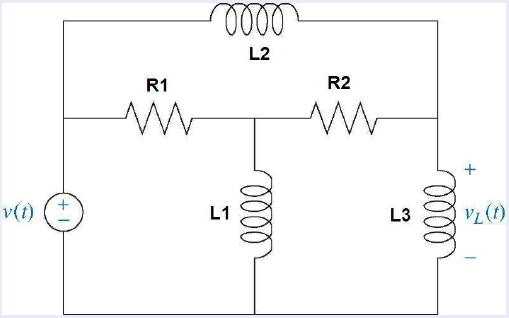
\includegraphics[scale = 0.5]{./images/circuit1.png}
		\caption{sistema dinâmico linear elétrico}
		\label{fig:circuit1}
	\end{subfigure}
	\hspace{1 cm}
  \begin{subfigure}[!htp]{0.5\textwidth}
		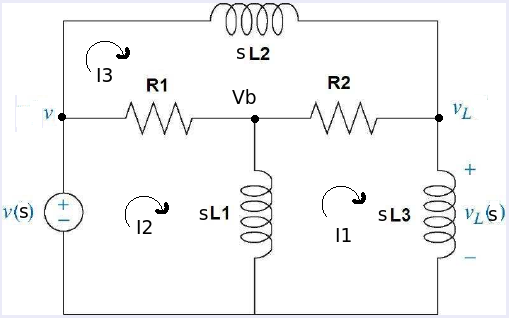
\includegraphics[scale = 0.5]{./images/circuit1-freq.png}
		\caption{sistema no domínio da frequência}
		\label{fig:circuit1-freq}
	\end{subfigure}
\end{figure}
\FloatBarrier
 

%@@@@@@@@@@@@@@@@@@@@@@@@@@@@@@@@@@@@@@@@@@@@@@@@@@@@@@@@@@@
%@@@@@@@@@@@@       PROCEDIMENTOS        @@@@@@@@@@@@@@@@@@@
%@@@@@@@@@@@@@@@@@@@@@@@@@@@@@@@@@@@@@@@@@@@@@@@@@@@@@@@@@@@
\newpage
\section{Descrição Experimental}
\paragraph{}Primeiramente resolvemos o seguinte sistema
de equações lineares:
\begin{displaymath}
  \left\{
       \begin{array}{l}
          x + y + 2z = 9 \\
          2x + 4y - 3z = 1 \\
          3x + 6y - 5z = 0        
      \end{array}
  \right.
\end{displaymath}
o script matlab para resolver esse sistema é apresentado a seguir:

\begin{lstlisting}[frame=single]

%entrando com o sistema na forma Ax = b

    A = [1 1 2;
        2 4 -3;
        3 6 -5];

    b = [9;
        1;
        0;];
disp('Resolvendo um sistema na forma A\b')
    x = A\b

disp('Resolvendo um sistema na forma A^(-1)*b')
    x = A^(-1)*b
\end{lstlisting}

\paragraph{}Vamos agora resolver a equação \ref{eq:crammerI1}
da introdução para determinar a função de transferência. O código
é apresentado a seguir:

\newpage

\begin{lstlisting}[frame=single]

%vamos salvar a saida de texto
    diary('exercicio2-output')
    diary on

% variaveis simbolicas
    syms L1 L2 L3 R1 R2 V s t


%entrando com a matriz dos coeficientes
    A = [ s*(L3+L1)+R2 -L1*s -R2; 
             -L1*s L1*s+R1 -R1;
             -R2 -R1 L2*s+R1+R2]

%entrando com a matriz Aj
%a primeira coluna(correspondente a I1) e substituida
    Aj = A;
    Aj(:,1) = [0;
              V;
              0]

 %calcula I1 e simplifica a expressao encontrada
     i1 = det(Aj)/det(A);
     i1 = simplify(i1)

 %calculamos a funcao de transferencia
     VL = i1*L3*s
     H = VL/V

 %agrupa termos semelhantes e mostra na tela
 %...de modo 'bonito'
     H = collect(H)
     pretty(H)
    
     diary off
\end{lstlisting}

\paragraph{}Por último, criamos uma rotina que irá receber
como parâmetros os valores dos componentes do circuito 
e retornar a função de transferência encontrada. O código
é mostrado a seguir. A rotina é semelhante ao código anterior,
por isso omitimos os comentários.
\newpage
\begin{lstlisting}[frame=single]
  function H = circuitSolver(R1, R2, L1, L2, L3)

diary('exercicio2b-output');
diary on;

		syms V s t;
		A = [ s*(L3+L1)+R2 -L1*s -R2; 
		         -L1*s L1*s+R1 -R1;
		         -R2 -R1 L2*s+R1+R2];
		Aj = A;
		Aj(:,1) = [0;
		          V;
		          0];

		 i1 = det(Aj)/det(A);
		 i1 = simplify(i1);
		 VL = i1*L3*s;
		 H = VL/V;
		 H = collect(H);
 diary off;
\end{lstlisting}

A função acima é salva em um arquivo 'circuitSolver.m'. O código 
a seguir testa o funcionamento da rotina para algumas entradas:

\begin{lstlisting}[frame=single]
      H = circuitSolver(1,1,1,1,1)
      H = circuitSolver(6,1,7,5,1)
\end{lstlisting}
%@@@@@@@@@@@@@@@@@@@@@@@@@@@@@@@@@@@@@@@@@@@@@@@@@@@@@@@@@@@
%@@@@@@@@@@@@@@@@@@@       DADOS      @@@@@@@@@@@@@@@@@@@@@@
%@@@@@@@@@@@@@@@@@@@@@@@@@@@@@@@@@@@@@@@@@@@@@@@@@@@@@@@@@@@
 \newpage
\section{Resultados}

\paragraph{}A saída dos códigos descritos é apresentada a seguir:

\begin{itemize}
  \item \textbf{resolvendo o sistema}
  \begin{lstlisting}[frame=single]
    A =

         1     1     2
         2     4    -3
         3     6    -5


    b =

         9
         1
         0

    Resolvendo um sistema na forma A\b

    x =

        1.0000
        2.0000
        3.0000

    Resolvendo um sistema na forma A^(-1)*b

    x =

        1.0000
        2.0000
        3.0000
      \end{lstlisting}

\item \textbf{achando a função de transferência}
\begin{lstlisting}[frame=single]
   
A =
 
[ R2 + s*(L1 + L3),     -L1*s,            -R2]
[            -L1*s, R1 + L1*s,            -R1]
[              -R2,       -R1, R1 + R2 + L2*s]
 
 
Aj =
 
[ 0,     -L1*s,            -R2]
[ V, R1 + L1*s,            -R1]
[ 0,       -R1, R1 + R2 + L2*s]
 
H = 
             2
((L1 L2 L3) s  + (L1 L3 R1 + L1 L3 R2) s + L3 R1 R2) /

                2
   ((L1 L2 L3) s  + (L1 L2 R1 + L1 L2 R2 + L1 L3 R1 + L1 L3 R2 
   + L2 L3 R1) s + L2 R1 R2 + L3 R1 R2)

\end{lstlisting}

Utilizando a função 'latex' do Matlab podemos obter o código LateX para a 
expressão acima. Temos : 

\begin{displaymath}
\hspace{-2 cm}  H = \frac{\left(\mathrm{L1}\, \mathrm{L2}\, \mathrm{L3}\right)\, s^2 + \left(\mathrm{L1}\, \mathrm{L3}\, \mathrm{R1} + \mathrm{L1}\, \mathrm{L3}\, \mathrm{R2}\right)\, s + \mathrm{L3}\, \mathrm{R1}\, \mathrm{R2}}{\left(\mathrm{L1}\, \mathrm{L2}\, \mathrm{L3}\right)\, s^2 + \left(\mathrm{L1}\, \mathrm{L2}\, \mathrm{R1} + \mathrm{L1}\, \mathrm{L2}\, \mathrm{R2} + \mathrm{L1}\, \mathrm{L3}\, \mathrm{R1} + \mathrm{L1}\, \mathrm{L3}\, \mathrm{R2} + \mathrm{L2}\, \mathrm{L3}\, \mathrm{R1}\right)\, s + \left(\mathrm{L2}\, \mathrm{R1}\, \mathrm{R2} + \mathrm{L3}\, \mathrm{R1}\, \mathrm{R2}\right)}
\end{displaymath}

\item \textbf{testando a rotina}
\begin{lstlisting}[frame=single]
>> H = circuitSolver(1,1,1,1,1)
 
H =
 
(s^2 + 2*s + 1)/(s^2 + 5*s + 2)
 
>> 
>> H = circuitSolver(6, 1, 7, 5, 1)
 
H =
 
(35*s^2 + 49*s + 6)/(35*s^2 + 324*s + 36)
\end{lstlisting}

\end{itemize}
%@@@@@@@@@@@@@@@@@@@@@@@@@@@@@@@@@@@@@@@@@@@@@@@@@@@@@@@@@@@
%@@@@@@@@@@@@@@       Análise         @@@@@@@@@@@@@@@@@@@@@@
%@@@@@@@@@@@@@@@@@@@@@@@@@@@@@@@@@@@@@@@@@@@@@@@@@@@@@@@@@@@
 \newpage
\section{Discussões e Conclusões}
\paragraph{} 
Na primeira etapa vimos como resolver rapidamente sistema lineares
com a notação matricial do matlab. Em seguida vimos como transformar
um circuito em um sistema matricial a ser resolvido.
Na terceira etapa rescrevemos o script anterior, mas na forma de 
uma função que reebe de entrada os parâmetros do ciruito.
As vantagens da codificação de rotinas para o matlab se torna
evidente quando um mesmo circuito precisa ser resolvido várias vezes.
Nesse caso, podemos apenas mudar alguns parâmetros de entrada 
de uma rotina e obter a nova resposta. O engenheiro então resolve 
o problema apenas uma vez e deixa para o computador a tarefa tediosa
dos cálculos repetitivos. 
%@@@@@@@@@@@@@@@@@@@@@@@@@@@@@@@@@@@@@@@@@@@@@@@@@@@@@@@@@@@
%@@@@@@@@@@@@@@       REFERÊNCIAS     @@@@@@@@@@@@@@@@@@@@@@
%@@@@@@@@@@@@@@@@@@@@@@@@@@@@@@@@@@@@@@@@@@@@@@@@@@@@@@@@@@@
\begin{thebibliography}{9}    
	 \bibitem{ADL-NISE}
  		Nise, N.S.
  		\emph{Engenharia de Sistemas de Controle}
 		 5ª ed.
		LTC, 2009.
	 \bibitem{ADL-OGATA}
  		Ogata, K.
  		\emph{Moder Control Engeeniring}
 		 5ª ed.
		Pearson, 2010.
 		 
\end{thebibliography}
\end{document}
